\documentclass[conference]{IEEEtran}
\usepackage[T1]{fontenc}
\usepackage{amsmath,amssymb}
\usepackage{graphicx}
\usepackage{booktabs}
\usepackage{xurl}
\usepackage[hidelinks]{hyperref}
\graphicspath{{../figures/}}

\newcommand{\repourl}{https://github.com/arvindermundraa/csce642-waymax-ppo}
\newcommand{\videourl}{VIDEO-URL-TO-BE-ADDED}
\newcommand{\pp}{\phantom{0}}

\begin{document}

\title{Learning Safe Closed-Loop Driving Policies\\ with PPO in the Waymax Simulator\\[6pt]
{\normalsize CSCE 642 Deep Reinforcement Learning, Texas A\&M University, final project report\\[2pt]
\textbf{Code:} \url{\repourl} \qquad \textbf{Video:} \url{\videourl}}}

\author{
\IEEEauthorblockN{Debmalya Chatterjee}
\IEEEauthorblockA{UIN 937005903\\
\textit{requested for consideration for Graduate}\\
\textit{Course Project Evaluation}}
\and
\IEEEauthorblockN{Arvinder Singh Mundra}
\IEEEauthorblockA{UIN 335007465\\
\textit{requested for consideration for Graduate}\\
\textit{Course Project Evaluation}}
}

\maketitle

\begin{abstract}
We train a Proximal Policy Optimization (PPO) agent that drives one car in closed loop
through real traffic scenes from the Waymo Open Motion Dataset, using the Waymax simulator,
and compare it on 288 held-out scenes with a hand-designed controller (pure pursuit with
Intelligent Driver Model speed control), Waymax's IDM policy and the logged human driver.
With the observation and reward from our proposal, PPO follows its route about as far as
the human did but collides in 28.6\% of scenes against 7.3\% for the controller, mostly
because it does not learn to wait in queues and at red lights. Policies trained on
replayed traffic collide less, not more, when the other cars react to them. Larger
penalties trade progress for safety and at the highest setting the agent stalls in
14.5\% of driving scenes. A follow-up that adds lead-vehicle features and a
time-to-collision penalty brings collisions down to 9.5\%, statistically
indistinguishable from the controller on replayed traffic, but the gain does not carry
over to reactive traffic. We report three seeds per setting, bootstrap confidence
intervals and paired tests throughout.
\end{abstract}

\section{Introduction}

Much reinforcement learning (RL) work on driving uses synthetic roads and scripted
traffic~\cite{dosovitskiy2017carla,kiran2022survey}. Real traffic is harder: roads curve
irregularly, intersections differ from one another, and other drivers behave like people.
The Waymo Open Motion Dataset (WOMD)~\cite{ettinger2021womd} and the Waymax
simulator~\cite{gulino2023waymax} make it possible to train and test a driving policy in
closed loop on recorded scenes with modest hardware. We wanted to see how far a plain
on-policy method gets in that setting, and to measure it honestly against something
simple.

Our question is: \emph{can a PPO policy with continuous steering and acceleration make
progress along its route in real WOMD scenes without crashing or leaving the road, and
how does it compare with a simple hand-designed controller?} We stated three hypotheses
in the proposal.
\begin{itemize}
\item \textbf{H1.} On held-out scenes, PPO has a lower collision and off-road rate than
the hand-designed controller at similar route progress.
\item \textbf{H2.} A policy trained against replayed traffic does worse when the other
cars are switched to reactive IDM agents.
\item \textbf{H3.} Raising the collision and off-road penalties lowers the failure rate
but costs progress, and if pushed too far the agent learns to stop and wait.
\end{itemize}

This is an application project, not a new algorithm. The short version of the result is
that H1 is not supported, H2 comes out reversed, and H3 is supported. PPO learns to
follow the route, but a short controller that tracks the gap to the vehicle ahead is
much safer. A failure analysis shows why, and a targeted change to the observation and
reward closes most of the gap on replayed traffic but not under reactive traffic.

What we built ourselves: the scene selection and caching, the environment wrapper around
Waymax (observation, action scaling, reward, termination), a vectorized reactive IDM
traffic model, PPO in JAX/Flax, the hand-designed controller, the evaluation protocol with
its statistics, a failure classifier and the rendering code. Section~\ref{sec:attribution}
lists what we took from others.

\section{Related Work}

\textbf{Data and simulation.} WOMD~\cite{ettinger2021womd} contains more than 100,000
real scenes recorded at 10\,Hz, mined for interactions such as merges and unprotected
turns, each with object tracks and a high-definition map. It was built for motion
forecasting, so each scene only records what the humans did. Waymax~\cite{gulino2023waymax}
turns these scenes into a closed-loop simulator written in JAX: the user controls any
subset of agents, and the others replay their logs or follow an IDM route-following
policy. It provides a bicycle dynamics model, collision and off-road metrics, and
benchmarks of imitation and RL planners. Two of its findings matter to us: route
information helps planning agents a great deal, and a DQN agent trained against replayed
traffic collided \emph{less} when evaluated against IDM agents, which is the opposite of
our H2. Waymax does not provide an observation design, a shaped reward or a ready-made
agent for our task, and we wrote those. CARLA~\cite{dosovitskiy2017carla} is the standard
synthetic alternative, with rendered sensors and scripted traffic; we chose recorded
scenes because the behavior of the other road users is real, at the cost of
bounding-box observations instead of sensor data.

\textbf{Policy gradient methods.} REINFORCE~\cite{williams1992reinforce} estimates the
gradient of expected return from sampled trajectories, and actor-critic methods reduce
its variance with a learned baseline~\cite{sutton2018rl}. Generalized advantage estimation
(GAE)~\cite{schulman2016gae} interpolates between one-step temporal-difference errors and
Monte Carlo returns with a parameter $\lambda$. PPO~\cite{schulman2017ppo} adds a clipped
surrogate objective that limits how far one update can move the policy, which allows
several epochs of minibatch updates per batch of experience. We use PPO because our
actions are continuous, it works with batched rollouts from many parallel environments,
and it tolerates changes to the reward and observation without retuning. Its cost is
that it is on-policy and needs many samples. Implementation details matter as much as
the algorithm: Engstrom et al.~\cite{engstrom2020implementation} show that code-level
choices such as normalization and learning-rate annealing account for much of PPO's
performance, and Andrychowicz et al.~\cite{andrychowicz2021matters} find the initial
action standard deviation among the choices that matter most, which matches our own
experience (Section~\ref{sec:hyper}). We followed the structure of CleanRL's
single-file continuous-action PPO~\cite{huang2022cleanrl} for these details and wrote our
own JAX version.

\textbf{Hand-designed driving.} The Intelligent Driver Model~\cite{treiber2000idm} sets a
vehicle's acceleration from its speed relative to a desired speed and from the gap and
closing speed to the vehicle ahead, with a few physically meaningful parameters. Pure
pursuit~\cite{coulter1992purepursuit} steers along the arc that passes through a point a
fixed distance ahead on the path. Our baseline controller combines the two. Unlike the
learned policy it encodes the designer's knowledge directly, which is exactly why it is
a useful reference: it shows what the task requires.

\textbf{Imitation and closed-loop RL for driving.} Behavior cloning for driving goes back
to ALVINN~\cite{pomerleau1989alvinn}. Its weakness is that small errors take the policy
to states the demonstrations never covered, and the errors compound; Ross et
al.~\cite{ross2011dagger} analyze this and correct it by querying the expert on the
learner's own states, which is not possible with a fixed log. Lu et
al.~\cite{lu2022imitation} combine imitation with RL on a large set of real driving
scenes and find that the RL term helps most in rare, difficult scenes. Peng et
al.~\cite{peng2024finetuning} pretrain a multi-agent behavior model on WOMD and fine-tune
it with RL in closed loop, lowering collision rates. Both start from large pretrained
models and far more data than we use. We train a single ego policy from scratch with a
compact observation, and our behavior-cloning stretch goal is a small-scale look at the
same question. Kiran et al.~\cite{kiran2022survey} survey deep RL for driving and note
that reward design and validation remain open problems, which is where most of our effort
went.

\textbf{Reward design and evaluation.} Shaping rewards can change what the optimal
policy is unless the shaping has a particular form~\cite{ng1999shaping}; our reward is
not potential-based, and Section~\ref{sec:hyper} describes two cases where the agent
exploited it. Henderson et al.~\cite{henderson2018matters} show how much deep RL
results vary across seeds and argue for reporting that spread, which we do with three
seeds per setting, bootstrap intervals~\cite{efron1993bootstrap} and McNemar's
test~\cite{mcnemar1947} on paired outcomes.

\section{Problem Formulation}

\subsection{Why the problem is sequential}
Every 0.1\,s the ego car observes its surroundings and chooses an acceleration and a
steering curvature. That choice determines where it is at the next step, which changes
the gaps to every other road user. The consequences are delayed: accelerating now gains
progress but can leave no room to brake behind a car that slows two seconds later, and
a small heading error on a curve grows until the car is off the road. The agent has to
trade progress against safety over the whole 8\,s episode, so it is a control problem
over a trajectory and not a sequence of independent decisions.

\subsection{Scenes}
We use one training shard and one validation shard of WOMD v1.1 in the format Waymax
reads: 478 training scenes and 288 held-out scenes. Each is 9.1\,s at 10\,Hz. Waymax
replays the first 1.1\,s as history and we control the remaining 80 steps. We keep every
scene. Scenes where the human covers less than 20\,m (queues, red lights, parked) are
\emph{waiting} scenes and the rest are \emph{driving} scenes; the held-out set has 168
driving and 120 waiting scenes. Each scene keeps the 64 objects that come closest to the
ego's logged path, the 3,000 map points closest to the route, and the traffic signals
that control lanes the logged ego drove along. The route the agent follows is the ego's
logged path resampled every meter and extended 30\,m past its end.

\subsection{Observation}
The policy sees a 50-dimensional vector: ego speed, heading error and lateral offset
relative to the route, fraction of the route covered, time left in the episode, and the
previous acceleration and curvature (7 values); five route points 5 to 25\,m ahead in the
ego frame (10); the next signal on the route as distance, red-or-not and presence (3);
and for each of the $K=5$ nearest objects within 50\,m the relative position and velocity
in the ego frame, a pedestrian-or-cyclist flag and a presence flag (30). Seeing only five
objects and one signal makes this a partially observable problem. Time left is in the
observation so that the fixed 80-step horizon does not break the Markov property of the
value function.

\subsection{Action and transition}
The action is a normalized pair $[a,\kappa]\in[-1,1]^2$, scaled to the bounds of Waymax's
invertible bicycle model, $\pm 6$\,m/s$^2$ of acceleration and $\pm 0.3$\,m$^{-1}$ of
curvature. The simulator applies the bicycle model to the ego. The other objects either
replay their logged trajectories (\emph{replay} traffic) or follow their logged paths
with IDM speed control and react to the ego (\emph{reactive} traffic,
Section~\ref{sec:idm}). A scene is sampled uniformly at each reset.

\subsection{Reward and termination}
\begin{equation}
r_t = w_p\,R^{\text{prog}}_t - w_c\,C^{\text{coll}}_t - w_o\,C^{\text{off}}_t - w_a\,C^{\text{ctrl}}_t .
\end{equation}
$R^{\text{prog}}_t$ is the distance gained along the route as a percentage of the logged
distance (at least 20\,m), so following the human through a driving scene earns about
100 per episode. Progress only counts up to 2\,m ahead of where the logged car was at
that step. $C^{\text{coll}}$ and $C^{\text{off}}$ are indicators from Waymax's overlap
check and its off-road check applied to the ego. $C^{\text{ctrl}}$ sums squared jerk
(scaled by 10\,m/s$^3$), squared curvature change (scaled by 0.02\,m$^{-1}$) and braking
beyond 3\,m/s$^2$, clipped at 10. The episode ends on a collision, on leaving the road, or
after 80 steps. We use three presets: \emph{progress} ($w_c=w_o=10$, $w_a=0.02$),
\emph{balanced} ($50$, $0.05$) and \emph{safety} ($200$, $0.1$), all with $w_p=1$.
Crossing an on-route stop line on red is measured but not penalized in these presets, so
that it is an outcome we can compare across methods.

\section{Methods}

\subsection{PPO}
The actor is a Gaussian policy $\pi_\theta(a\,|\,s)$ whose mean comes from an MLP with two
hidden layers of 256 tanh units and whose log standard deviation is a state-independent
parameter. The critic $V_\phi(s)$ is a separate MLP of the same size. Each update
collects 64 steps from 64 parallel environments (4,096 transitions), computes advantages
with GAE,
\begin{equation}
\hat{A}_t=\sum_{l\ge 0}(\gamma\lambda)^l\,\delta_{t+l},\qquad
\delta_t=r_t+\gamma V_\phi(s_{t+1})-V_\phi(s_t),
\end{equation}
and runs 4 epochs over 8 minibatches on the clipped objective
\begin{equation}
L(\theta)=\mathbb{E}_t\!\left[\min\!\big(\rho_t\hat{A}_t,\;
\mathrm{clip}(\rho_t,1-\epsilon,1+\epsilon)\hat{A}_t\big)\right],
\end{equation}
with $\rho_t=\pi_\theta(a_t|s_t)/\pi_{\theta_\text{old}}(a_t|s_t)$, plus a squared-error
value loss. Advantages are normalized per minibatch, observations are normalized with
running statistics, gradients are clipped, and the learning rate is annealed linearly to
zero. The rollout is a \texttt{jax.lax.scan} over vectorized environments, so one whole
update is a single compiled function; finished episodes are reset to a new random scene
inside the scan. Every run uses 2M environment steps (488 updates). Evaluation uses the
mean action.

\subsection{Reference methods}
\textbf{Hand-designed controller.} Steering is pure pursuit toward the route point a
distance $\ell=\mathrm{clip}(4+0.8v,\,5,\,20)$\,m ahead, $\kappa=2y_\ell/\ell^2$ with
$y_\ell$ the lateral offset of that point in the ego frame. Speed follows IDM,
\begin{equation}
\dot v=a_{\max}\Big[1-\big(\tfrac{v}{v_0}\big)^4-\big(\tfrac{s^*}{g}\big)^2\Big],\;\;
s^*=s_0+vT+\tfrac{v\,\Delta v}{2\sqrt{a_{\max}b}},
\end{equation}
where $g$ is the gap to the nearest object ahead within $\pm 2$\,m laterally, or to the
stop line of a red signal on the route, whichever is closer. The desired speed $v_0$ is
the mean logged speed in the scene plus 1\,m/s.
\textbf{IDM ego.} Waymax's \texttt{IDMRoutePolicy} controlling the ego along its logged
path. \textbf{Logged human.} The recorded trajectory replayed through our wrapper, as a
reference for how the scene was actually driven and as a check of the wrapper itself.

\subsection{Reactive traffic}\label{sec:idm}
Waymax's \texttt{IDMRoutePolicy} ran at about 75 environment steps per second with 64
objects on our hardware, against about 3,000 for replay, which would have made one
training run with reactive traffic take more than seven hours. We wrote the same behavior
as a vectorized Waymax actor: every car follows its own logged path and sets its speed
with IDM from the nearest object ahead in its lane, the ego included, with its highest
logged speed as desired speed. It runs at about 2,200 steps per second. It differs from
Waymax's policy in one respect: a car is handed back to log replay when it reaches the
end of its recorded path, so it never drives straight off the map. We check it against
Waymax's policy in Section~\ref{sec:h2}.

\section{Experimental Setup}

\textbf{Runs.} Table~\ref{tab:runs} lists the trained settings. All use the same PPO
configuration and three seeds.

\begin{table}[t]
\caption{Trained settings (three seeds each, 2M steps).}\label{tab:runs}
\centering\small
\begin{tabular}{@{}lll@{}}
\toprule
Name & Reward & Differs from balanced in \\
\midrule
balanced & 50/50 & (main setting) \\
progress & 10/10 & lower penalties \\
safety & 200/200 & higher penalties \\
IDM-trained & 50/50 & reactive traffic in training \\
BC$\rightarrow$PPO & 50/50 & initialized from behavior cloning \\
rich obs. & 50/50 & $K=10$ and 16 road-edge points \\
intersections & 50/50 & trained on 100 intersection scenes \\
lead/TTC & 50/50 + terms & Section~\ref{sec:improved} \\
\bottomrule
\end{tabular}
\end{table}

\textbf{Metrics.} Every method runs on the same 288 held-out scenes. Per episode we record
collision, off-road and red-light violation (any time in the episode); route progress
(distance covered along the route divided by the logged distance, at least 20\,m);
success (no collision, no off-road event and at least 80\% of the distance the human
covered, minus 1\,m, which is meaningful for both driving and waiting scenes); return
under the balanced reward; and mean absolute jerk and curvature change.

\textbf{Statistics.} For PPO we report the mean and standard deviation across the three
seeds and a 95\% bootstrap confidence interval over (seed, scene): scenes are resampled
with replacement 2,000 times, the same resample is used for every seed, and the mean is
taken over seeds and scenes. The reference methods are deterministic, so their interval
comes from resampling scenes. Comparisons between two methods are paired by scene:
McNemar's exact test on per-scene collision (for PPO, the majority outcome over seeds)
and a paired bootstrap on the difference in success rate.

\textbf{Failure types.} Each failure is labeled at the step it happens with simple
geometric rules: \emph{struck from behind} (the nearest object is behind the ego, which
under replay is a recorded car driving into a slower ego), \emph{collision while
turning} (route or ego curvature above 0.02\,m$^{-1}$), \emph{rear-end} (nearest object
ahead within $\pm 2$\,m laterally), \emph{other collision}, \emph{off-road on a curve},
\emph{off-road on a straight}, and \emph{stalled} (no failure but under half of the
logged distance covered in a driving scene).

\section{Results}

\subsection{First result: one scene}
As the proposal's first milestone we trained PPO on a single training scene (a 28\,m
path with a 50$^\circ$ turn and 14 objects within 30\,m) for 200,000 steps. The learned
policy completes it without collision or off-road event and covers 31\,m, and so does
the hand-designed controller (30\,m). This confirmed that the wrapper, reward and PPO
were working before we scaled up.

\subsection{H1: PPO against the hand-designed controller}

\begin{table*}[t]
\caption{Held-out scenes, replayed traffic. PPO rows are mean $\pm$ standard deviation
over three seeds; brackets are 95\% bootstrap confidence intervals.}\label{tab:main}
\centering\small
\begin{tabular}{@{}lccccc@{}}
\toprule
Method & Collision \% & Off-road \% & Ran red \% & Progress \% & Success \% \\
\midrule
Logged human & 0.3 [0.0, 1.0] & 1.7 & 1.4 & 67.9 & 97.9 [96.2, 99.3] \\
IDM (Waymax) ego & 13.2 [9.7, 17.4] & 8.3 & 5.2 & 92.9 & 77.1 [72.2, 81.6] \\
Hand-designed & 7.3 [4.5, 10.4] & 3.8 & 2.8 & 74.4 & 85.8 [81.6, 89.6] \\
\midrule
PPO progress & $54.2\pm2.8$ [48.7, 59.4] & $11.7\pm0.7$ & $13.3\pm0.3$ & $97.6\pm0.6$ & $32.1\pm4.6$ [27.3, 36.6] \\
PPO balanced & $28.6\pm1.1$ [24.2, 33.1] & $4.2\pm0.3$ & $10.5\pm1.7$ & $83.2\pm1.4$ & $66.6\pm0.9$ [61.7, 71.3] \\
PPO safety & $21.4\pm1.3$ [17.7, 25.3] & $4.6\pm1.7$ & $5.2\pm0.3$ & $61.4\pm0.8$ & $53.5\pm3.7$ [49.0, 58.3] \\
PPO balanced, IDM-trained & $33.0\pm2.3$ [28.1, 38.2] & $6.0\pm0.3$ & $6.7\pm0.6$ & $73.7\pm2.5$ & $54.6\pm3.4$ [49.5, 59.7] \\
\midrule
PPO + lead/TTC/red terms & $9.5\pm2.7$ [6.8, 12.4] & $7.8\pm1.2$ & $2.8\pm0.5$ & $90.1\pm3.3$ & $81.8\pm2.8$ [78.1, 85.4] \\
\quad same, route frame & $11.1\pm1.0$ [8.2, 14.1] & $6.5\pm0.4$ & $3.0\pm0.3$ & $87.3\pm1.1$ & $80.7\pm1.8$ [76.9, 84.4] \\
\bottomrule
\end{tabular}
\end{table*}

\begin{figure}[t]
\centering
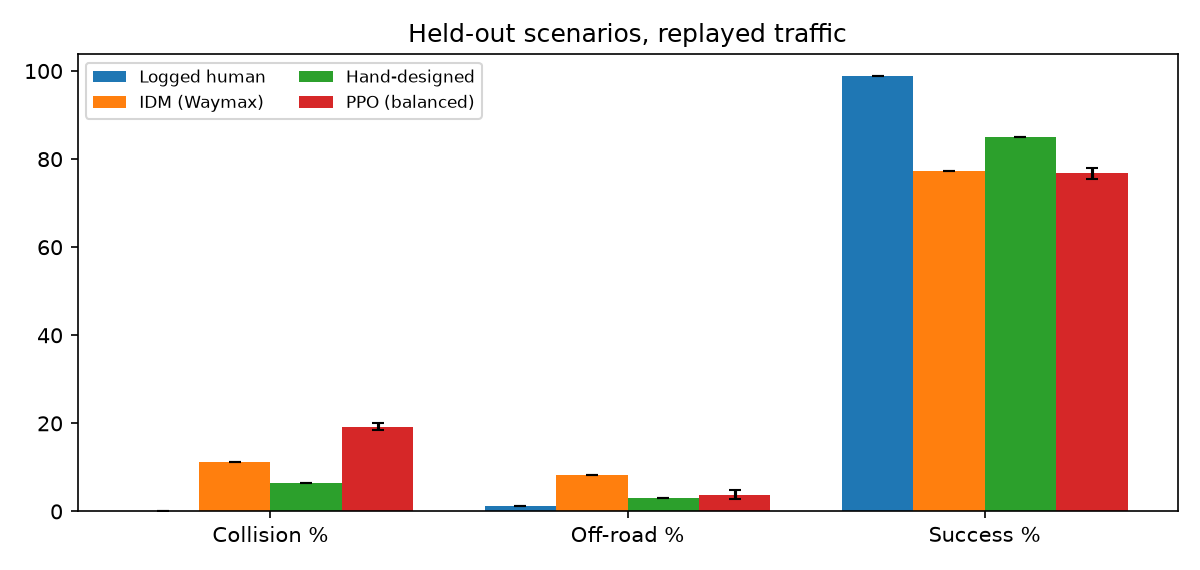
\includegraphics[width=\columnwidth]{main_comparison.png}
\caption{Held-out scenes with replayed traffic; error bars are 95\% bootstrap
intervals.}\label{fig:main}
\end{figure}

Table~\ref{tab:main} and Fig.~\ref{fig:main} give the main comparison. \textbf{H1 is not
supported.} With the balanced reward PPO collides in $28.6\pm1.1$\% of held-out scenes
against 7.3\% for the controller. Paired by scene, PPO collides alone in 68 scenes and
the controller alone in 9 (McNemar $p<0.001$), and PPO's success rate is 19.2 points
lower (95\% CI $[-24.3,-13.5]$). Off-road rates are close (4.2\% and 3.8\%). None of the
four settings trained under the original design beats the controller on collisions.

\begin{table}[t]
\caption{Driving and waiting scenes separately (replayed traffic).}\label{tab:split}
\centering\small
\begin{tabular}{@{}lcccc@{}}
\toprule
 & \multicolumn{2}{c}{Driving (168)} & \multicolumn{2}{c}{Waiting (120)} \\
Method & Coll.\,\% & Succ.\,\% & Coll.\,\% & Succ.\,\% \\
\midrule
Logged human & 0.0 & 98.8 & 0.8 & 96.7 \\
Hand-designed & 7.7 & 85.1 & 6.7 & 86.7 \\
PPO progress & 38.9 & 50.4 & 75.6 & \pp6.4 \\
PPO balanced & 15.7 & 80.4 & 46.7 & 47.2 \\
PPO safety & 21.4 & 44.6 & 21.4 & 65.8 \\
PPO + lead/TTC & \pp8.5 & 83.5 & 10.8 & 79.4 \\
\bottomrule
\end{tabular}
\end{table}

Table~\ref{tab:split} shows where the gap comes from. In driving scenes the balanced
policy covers 98.3\% of the logged route against 95.6\% for the controller, with 15.7\%
collisions against 7.7\% and 80.4\% success against 85.1\%. In waiting scenes it collides
in 46.7\% of episodes and runs a red light in 21.9\%, against 6.7\% and 5.0\%. The policy
did not learn to stay put when the human did.

\subsection{H2: replayed against reactive traffic}\label{sec:h2}

\begin{table}[t]
\caption{Collision rate (\%) by training and evaluation traffic.}\label{tab:h2}
\centering\small
\begin{tabular}{@{}lcc@{}}
\toprule
Method & Replay eval & IDM eval \\
\midrule
Logged human & 0.3 & 6.6 \\
Hand-designed & 7.3 & 7.3 \\
PPO balanced (replay-trained) & $28.6\pm1.1$ & $26.3\pm0.6$ \\
PPO safety (replay-trained) & $21.4\pm1.3$ & $14.0\pm1.3$ \\
PPO balanced (IDM-trained) & $33.0\pm2.3$ & $23.8\pm0.4$ \\
\bottomrule
\end{tabular}
\end{table}

\textbf{H2 does not hold; the effect goes the other way} (Table~\ref{tab:h2}). Under
reactive traffic the replay-trained balanced policy collides in 26.3\% of scenes instead
of 28.6\%, and the safety policy in 14.0\% instead of 21.4\%. Reactive cars brake for an
ego that is slower or closer than the human was, which forgives exactly the mistakes
that replayed cars punish. The controller is unchanged at 7.3\%, while the replayed
human trajectory goes from 0.3\% to 6.6\% because its fixed motion no longer matches cars
that now drive differently. Policies trained with reactive traffic collide a little
less under it (23.8\%) but more on replay (33.0\%): training against forgiving traffic
does not transfer to the recorded one. This is the same pattern Gulino et
al.~\cite{gulino2023waymax} report for DQN.

Our vectorized IDM agrees with Waymax's \texttt{IDMRoutePolicy} on the per-scene
collision outcome in 83 to 87\% of scenes for the three methods we checked, but Waymax's
version produces more collisions for each (14.6\% against 6.6\% for the logged human),
partly because its cars keep driving straight after their recorded path ends. The
direction of the H2 result is the same under both.

\subsection{H3: reward study}

\begin{figure}[t]
\centering
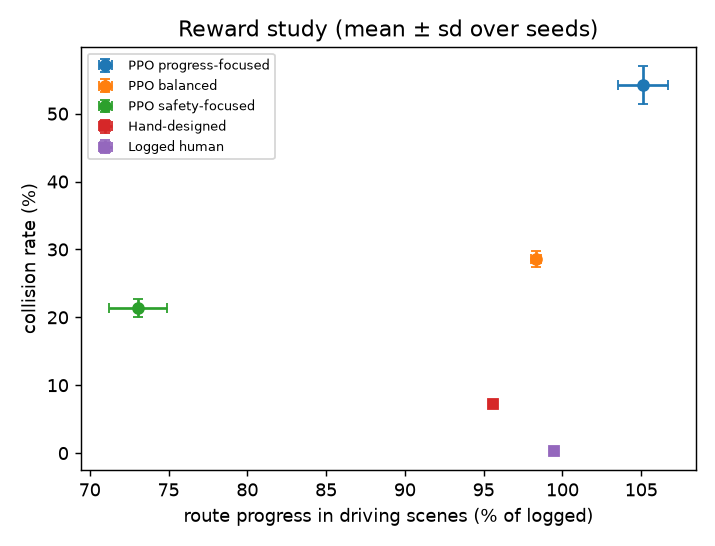
\includegraphics[width=0.85\columnwidth]{reward_study.png}
\caption{Collision rate against progress in driving scenes for the three reward presets
and two references (mean $\pm$ sd over seeds).}\label{fig:reward}
\end{figure}

\textbf{H3 is supported} (Fig.~\ref{fig:reward}). As the collision and off-road weight
goes from 10 to 50 to 200, collisions fall from 54.2\% to 28.6\% to 21.4\% and progress
in driving scenes falls from 105.1\% to 98.3\% to 73.1\% of the logged route.
Stop-and-wait appears only at the highest penalty: the safety policy stalls in 14.5\% of
driving scenes (17.3\%, 11.9\% and 14.3\% for the three seeds) and no other setting stalls
at all. It is also the only original setting that copes with waiting scenes (21.4\%
collisions against 46.7\% for balanced), so the caution that helps when the human waited
costs progress when the human drove, and its overall success rate (53.5\%) is below the
balanced policy's (66.6\%) despite fewer collisions. The control weight also differs
between presets, so the study varies a reward \emph{setting}, not one weight in
isolation.

\subsection{Failure analysis and smoothness}

\begin{figure}[t]
\centering
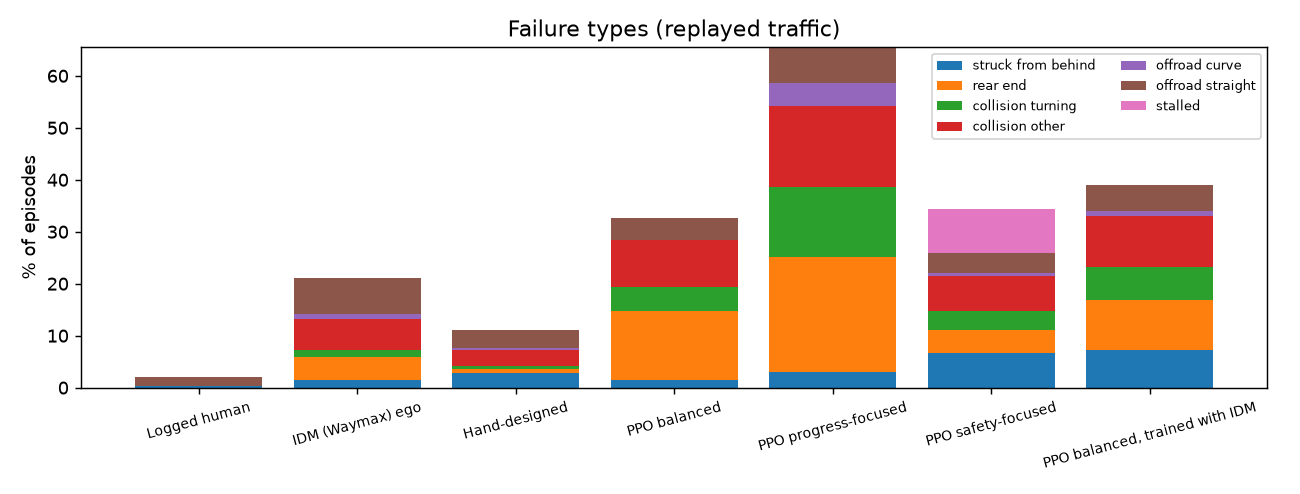
\includegraphics[width=\columnwidth]{failure_types.png}
\caption{Failure types as a share of episodes (replayed traffic, pooled over
seeds).}\label{fig:fail}
\end{figure}

Fig.~\ref{fig:fail} breaks failures down by type. For the balanced policy the most common
failure is running into the vehicle ahead (13.2\% of episodes), often by creeping into a
stopped queue, followed by other collisions (9.1\%), collisions while turning (4.7\%)
and leaving a straight road (4.2\%). Its median speed at failure is 5.2\,m/s, and 5.7\% of
its collisions involve a pedestrian or cyclist. The controller's most common collision
is a replayed car running into it from behind (2.8\%), which is an artifact of log
replay when the ego is slower than the human was, not a mistake by the controller. The
safety policy is struck from behind more often (6.6\%) for the same reason.

PPO also drives less smoothly than every reference: mean absolute jerk of 3.6\,m/s$^3$
for the balanced policy against 1.8 for the controller and 1.3 for the human, and
curvature changes about 25 times the controller's, visible in the videos as constant
small steering corrections.

\textbf{Checking the labels.} We checked the failure types by eye on 70 sampled episodes,
ten per type, drawn from the three reward settings (seed 0) and the controller, and
agreed with the label in 44. \emph{Struck from behind} (10/10), \emph{off-road on a
straight} (9/10) and \emph{rear-end} (8/10) hold up. \emph{Collision while turning} does
not (3/10): seven of the ten were the ego going straight into a vehicle ahead or a
crossing vehicle, labeled as turning because the policy's own steering corrections push
its curvature over the threshold. Three of ten \emph{other collisions} were rear-ends
too, so the rear-end share reported for PPO is an undercount. Four of ten \emph{stalled}
episodes were still moving slowly at the end, so that count mixes stopping with
hesitant driving. \emph{Off-road on a curve} (1/10) turned out to be mostly something
else: the progress policy driving past the end of the logged path, where the route is a
straight 30\,m extension that need not stay on the road. Table~\ref{tab:offroad} splits
off-road events accordingly. Every method, the logged human included, starts outside
the mapped road in 1.4\% of scenes, and within the logged path the rates are low and
close together. We kept the classifier as it was and report these error rates with it;
the hypothesis tests do not use the failure types.

\begin{table}[t]
\caption{Where off-road events happen (\% of episodes, replayed traffic).}\label{tab:offroad}
\centering\small
\begin{tabular}{@{}lcccc@{}}
\toprule
Method & All & Start & Past path & Within \\
\midrule
Logged human & \pp1.7 & 1.4 & 0.0 & 0.3 \\
Hand-designed & \pp3.8 & 1.4 & 1.4 & 1.0 \\
PPO progress & 11.7 & 1.4 & 8.4 & 1.9 \\
PPO balanced & \pp4.2 & 1.4 & 1.5 & 1.3 \\
PPO safety & \pp4.6 & 1.4 & 1.0 & 2.2 \\
PPO + lead/TTC & \pp7.8 & 1.4 & 4.7 & 1.6 \\
\quad same, route frame & \pp6.5 & 1.4 & 2.7 & 2.4 \\
\bottomrule
\end{tabular}
\end{table}

\subsection{Stretch goals}

\begin{table}[t]
\caption{Stretch goals, replayed traffic, all 288 scenes.}\label{tab:stretch}
\centering\small
\begin{tabular}{@{}lccc@{}}
\toprule
Method & Coll.\,\% & Off-road\,\% & Succ.\,\% \\
\midrule
Behavior cloning (BC) & 38.5 & 42.7 & 14.9 \\
PPO balanced & $28.6\pm1.1$ & $4.2\pm0.3$ & $66.6\pm0.9$ \\
BC$\rightarrow$PPO & $28.4\pm2.6$ & $5.1\pm0.4$ & $64.8\pm3.5$ \\
PPO, $K{=}10$ + road edges & $34.5\pm2.6$ & $5.9\pm0.9$ & $56.2\pm2.8$ \\
PPO, intersections only & $33.4\pm1.8$ & $10.0\pm1.1$ & $55.6\pm2.3$ \\
\bottomrule
\end{tabular}
\end{table}

\textbf{Behavior cloning.} We recovered expert actions from the logs with the bicycle
model's inverse dynamics (38,240 state-action pairs) and regressed them from the same
observation. The fit is good (mean squared error 0.003) but in closed loop the cloned
policy collides in 38.5\% of scenes and leaves the road in 42.7\%: the compounding-error
problem described by Ross et al.~\cite{ross2011dagger}. Starting PPO from the cloned
policy ends where PPO from scratch does (Table~\ref{tab:stretch}), so with this budget
the warm start neither helps nor hurts.
\textbf{Richer observation.} Ten neighbors and 16 road-edge points make results worse
on every seed. More inputs made the problem harder to learn in 2M steps, not easier.
\textbf{Harder slice.} Policies trained only on the 100 training scenes where the ego
turns or crosses a signal's stop line collide less on the 45 held-out scenes of that
kind than the policy trained on everything ($13.3\pm3.1$\% against $18.5\pm2.8$\%) but
leave the road more (11.9\% against 3.7\%), and their success rate is no better (72.6\%
against 76.3\%). Over all scenes they are worse. A fifth of the training set is not
enough to learn the slice well.

None of the stretch policies shows stop-and-wait (stalled in at most 1\% of driving
scenes; 2.4\% for behavior cloning). Under reactive traffic their order is unchanged:
$27.7\pm1.9$\% collisions for BC$\rightarrow$PPO, $28.7\pm4.0$\% for the richer observation
and $32.1\pm0.7$\% for the intersection-trained policy, against 26.3\% for balanced.

\subsection{Improving the policy}\label{sec:improved}

The failure analysis pointed at a missing input. The controller avoids rear-end
collisions and red lights because it tracks the gap to whatever is ahead in its lane.
We gave the policy the same information and made the reward say what the evaluation
measures: three extra observation values (gap, closing speed and time to collision to the
nearest object ahead within $\pm2$\,m, or to a red stop line), a penalty of up to 2 per
step when time to collision drops below 2\,s while moving, a penalty of 50 for crossing
a stop line on red, and a control weight of 0.1 instead of 0.05. Nothing else changed.

Over three seeds on replayed traffic this cuts collisions from 28.6\% to $9.5\pm2.7$\%
and raises success from 66.6\% to $81.8\pm2.8$\% (last rows of Table~\ref{tab:main};
paired against balanced: 66 scenes where only the balanced policy collides against 7,
success $+15.3$ points, CI $[10.3, 20.3]$). The gain is where the analysis said it would
be: in waiting scenes collisions fall from 46.7\% to 10.8\% and red-light violations from
21.9\% to 4.7\%, rear-end collisions fall from 13.2\% to 1.4\% of episodes, and jerk falls
from 3.6 to 2.3\,m/s$^3$. Against the hand-designed controller the collision difference
is gone: each collides alone in 13 scenes (McNemar $p=1.0$). Success is still 3.9 points
lower (CI $[-8.2, 0.2]$), mostly because the new policy leaves the road more often
(7.8\% against 3.8\%). Most of that difference is overrun: the new policy drives further
than the human did, and 4.7\% of its episodes leave the road after the end of the logged
path, against 1.4\% for the controller, while within the logged path the rates are 1.6\%
and 1.0\% (Table~\ref{tab:offroad}). Fig.~\ref{fig:frames} shows three scenes before and
after.

\begin{figure}[t]
\centering
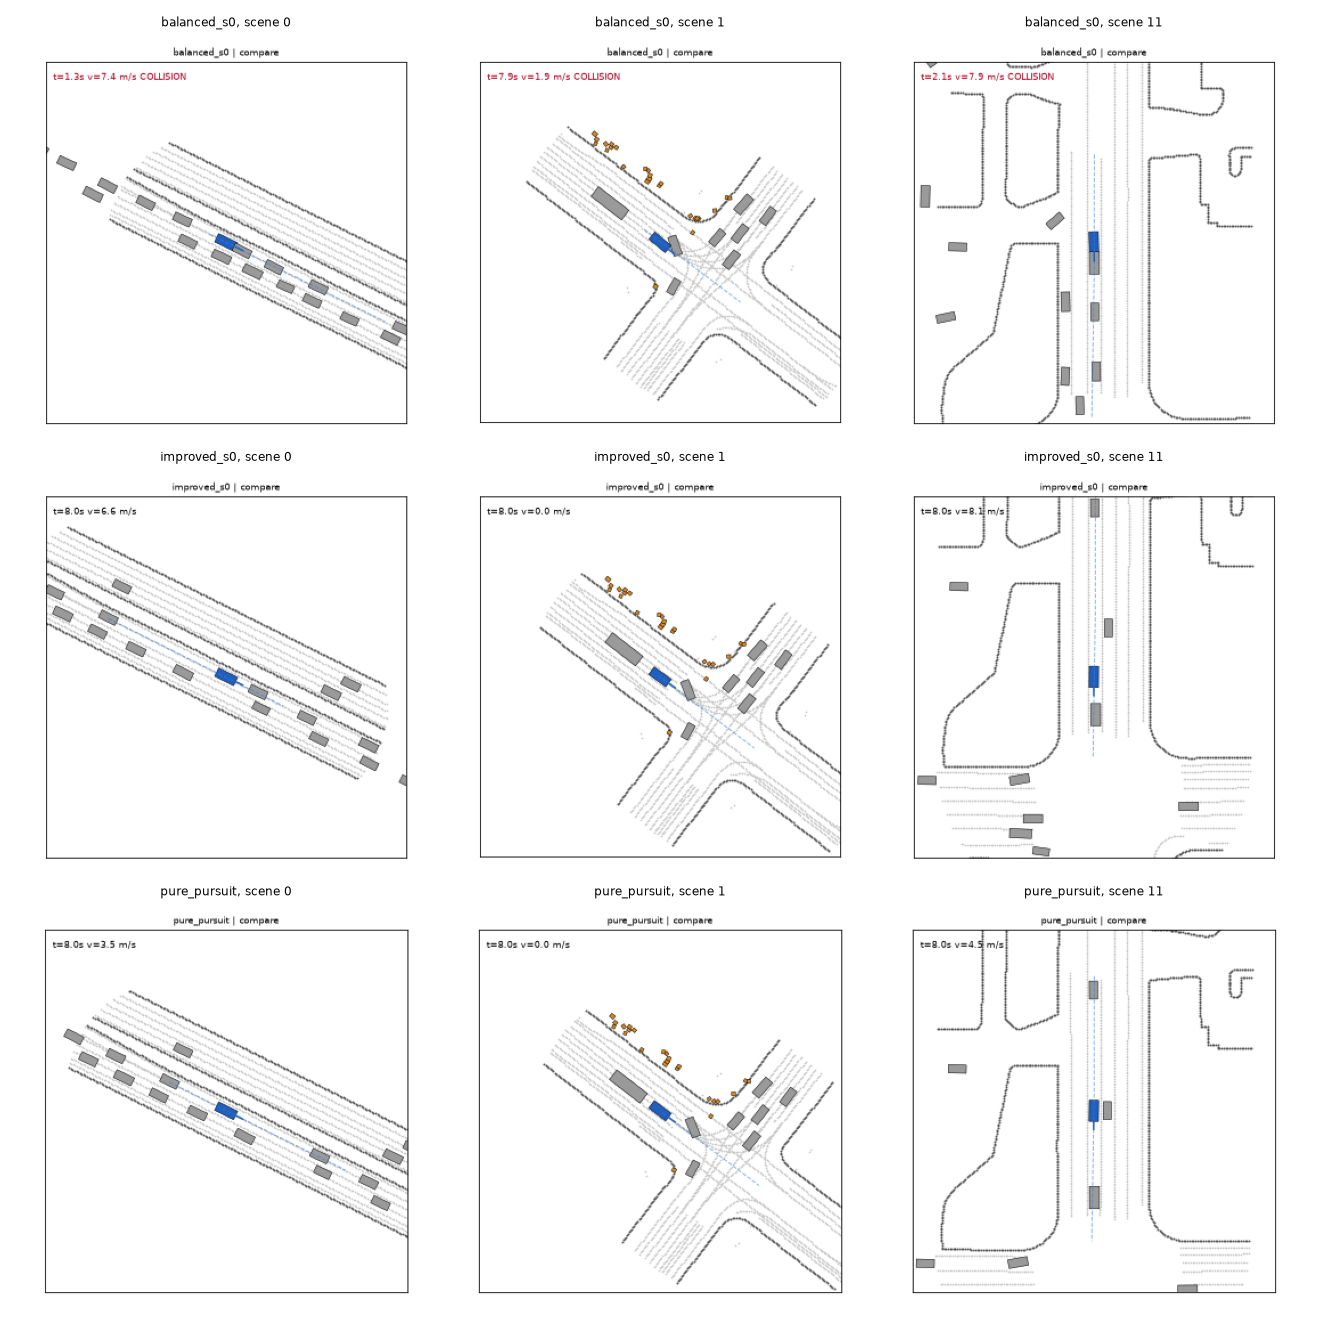
\includegraphics[width=\columnwidth]{improved_frames.png}
\caption{Last step of three held-out scenes for the balanced policy (top), the policy
with lead-vehicle terms (middle) and the hand-designed controller (bottom). The ego is
blue.}\label{fig:frames}
\end{figure}

Before we had that breakdown, the extra off-road exits looked like a loophole. The first
version measured ``ahead'' in
the ego's own frame, so steering out of the lane makes a stopped car leave the 2\,m band
and removes the penalty. A second version measures gap and closing speed along the route.
It lowers off-road exits (6.5\%, with overrun down from 4.7\% to 2.7\%) but raises
collisions slightly (11.1\%), and the two
versions are not significantly different (13 against 7 scenes, $p=0.26$).

Two caveats. First, the gain does not carry over to reactive traffic: under IDM the two
versions collide in 21.8\% and 19.7\% of scenes, only modestly below the balanced policy
(26.3\%) and far above the controller (7.3\%), with most of the extra collisions being
rear-ends in waiting scenes. We have not isolated the cause; one candidate is that our
IDM agents restart stopped cars toward their highest logged speed, a pattern the policy
never saw in training. Second, these changes were designed after looking at failures on
the held-out scenes, so their numbers are a second look at the same scenes and not a
fresh test. We keep them apart from the hypothesis tests for that reason.

\section{Discussion}

\textbf{What worked.} PPO from scratch, on a CPU, with 2M steps and a 50-number
observation, learns to follow routes through real intersections with an off-road rate
close to a hand-designed controller's. The JAX formulation made that budget possible:
about 3,000 environment steps per second on the two-core machine we trained on, with
the whole update compiled. The evaluation design held up. Splitting scenes into driving and waiting,
typing the failures and pairing methods by scene turned an unexplained collision rate
into a specific diagnosis, and the fix that the diagnosis suggested cut collisions by
two thirds.

\textbf{What did not.} The policy we proposed is clearly less safe than a simple
controller. With five nearest objects in the observation and a progress reward, the
agent has to infer ``there is a stopped car in my lane'' from raw relative positions,
and in 2M steps it does not; adding more raw inputs made it worse. The reward needed
several corrections that were each a response to the agent exploiting it (driving
faster than the human, creeping into queues, running on past where the human stopped), which is
the reward design problem in practice: the agent optimizes the reward we wrote, not the
behavior we meant. The learned policies are also
jerky, and even the improved one is not robust to a change in how other cars behave.
With hindsight H1 was optimistic. A controller that encodes the two rules that matter
(follow the path, keep a gap) is a strong baseline, and RL had to rediscover those rules
from a sparse penalty.

\textbf{What the traffic model does to the conclusions.} H2 taught us that a lower
collision rate under reactive traffic says as much about how forgiving the traffic
model is as about the policy. Neither traffic model is right: replayed cars drive into a
slow ego, and IDM cars never change lanes or yield at crossings.

\textbf{Limitations.} One shard per split and 2M steps per run. The hand-designed
controller's desired speed and the policy's progress feature both use the length of the
logged trajectory, which a deployed planner would not have. Red-light attribution is a
geometric heuristic, and the failure types were right in about two thirds of the
episodes we checked. Off-road events after the end of the logged path depend on a
straight route extension. The IDM ego baseline uses state dynamics and is not bound by the
bicycle model. The policy sees only five objects and one signal. The reference methods
are deterministic, so they have no seed variance to compare against. The follow-up in
Section~\ref{sec:improved} was designed on the evaluation scenes.

\section{Parameters and How We Chose Them}\label{sec:hyper}

We did not run a hyperparameter search. Table~\ref{tab:hyper} lists the values. Most
were the first values we tried; three were changed after an observed failure, described
below.

\begin{table}[t]
\caption{Parameter values and where they came from.}\label{tab:hyper}
\centering\small
\begin{tabular}{@{}p{0.33\columnwidth}p{0.25\columnwidth}p{0.32\columnwidth}@{}}
\toprule
Parameter & Value & Source \\
\midrule
Learning rate & $3\times10^{-4}$, decayed & CleanRL default \\
$\gamma$, $\lambda$, clip $\epsilon$ & 0.99, 0.95, 0.2 & CleanRL default \\
Value coef., grad. clip & 0.5, 0.5 & CleanRL default \\
Entropy coef. & 0 & CleanRL default \\
Envs $\times$ steps & $64\times64$ & first value tried \\
Epochs, minibatches & 4, 8 & first value tried \\
Hidden units & $2\times256$ & first value tried \\
Reward scale & 0.1 & first value tried \\
Initial log std & $-1.6$ & changed once \\
Progress cap & 2\,m & changed twice \\
Objects per scene & 64 & changed once \\
Penalties $w_c{=}w_o$ & 10, 50, 200 & chosen to differ clearly \\
TTC limit, $w_\text{ttc}$, $w_\text{red}$ & 2\,s, 2, 50 & first value tried \\
\bottomrule
\end{tabular}
\end{table}

\textbf{Initial policy standard deviation.} With an initial log standard deviation of
$-0.5$ (a standard deviation of 0.6 in normalized action units) the steering noise alone
made the car weave, and training stalled near 40\% collisions. We lowered it once to
$-1.6$ (about 0.2) and kept that.
\textbf{Progress cap.} Our first runs had no cap, and the agent learned to drive faster
than the human and collided more. A cap 5\,m ahead of the logged car still let it creep
into stopped queues. We settled on 2\,m, the third value.
\textbf{Objects per scene.} Waymax's loader keeps the first $N$ objects in file order.
With $N=32$ that left out about five of the roughly 19 objects that pass within 30\,m of
the ego; we load all 128 and keep the 64 closest to the ego's path, which leaves out 0.3
on average.
\textbf{Reward presets.} The three presets were chosen in advance as clearly different
settings, as the proposal said, and were not tuned. The terms in
Section~\ref{sec:improved} were set once.

\section{Code and Attribution}\label{sec:attribution}

All code is in one notebook in the repository, saved with the outputs of the full run;
per-scene results, summary tables, training logs and figures are tracked alongside it.

\textbf{Used from others.} The Waymax simulator~\cite{gulino2023waymax}, including its
data loader, bicycle and state dynamics, overlap and off-road metrics, inverse dynamics
and \texttt{IDMRoutePolicy}; the WOMD scenes~\cite{ettinger2021womd}; and JAX, Flax and
Optax. Our PPO follows the structure and default hyperparameters of CleanRL's
\texttt{ppo\_continuous\_action.py}~\cite{huang2022cleanrl} but is written by us in JAX;
no CleanRL code is copied. IDM~\cite{treiber2000idm} and pure
pursuit~\cite{coulter1992purepursuit} are published models that we implemented.

\textbf{Written by us.} Scene selection, route construction and signal attribution; the
environment wrapper, observation and reward; the vectorized reactive IDM actor; PPO; the
hand-designed controller; behavior cloning; the evaluation, statistics, failure
classifier and rendering.

This work was made using the Waymo Open Dataset, provided by Waymo LLC under the Waymo
Dataset License Agreement for Non-Commercial Use.

\section{Conclusion}

In real WOMD traffic a compact PPO policy learns to drive along its route about as far
as the human did, but with the observation and reward we proposed it is clearly less
safe than pure pursuit with IDM speed control, mostly because it does not learn when to
wait. Larger penalties reduce collisions at the cost of progress and eventually produce
the stop-and-wait behavior we anticipated. Switching to reactive traffic makes
replay-trained policies look safer, not worse. Giving the policy an explicit lead-vehicle
signal and a time-to-collision term closes the collision gap to the controller on
replayed traffic but not under reactive traffic, so the remaining difference between
learned and hand-designed driving here is robustness, not average-case safety. If we
continued, we would train with a mix of traffic models, evaluate the follow-up on fresh
scenes, and replace the five-nearest-objects input with an encoder over all nearby
objects.

\bibliographystyle{IEEEtran}
\bibliography{refs}

\end{document}
